\section{Resuelva el siguiente p.p.l.}
\begin{tabular}{|l|l|}
\hline
Max & 5x_1+4x_2        \\ \hline
s.a & x_1+2x_2 \leq 6  \\ \hline
    & -2x_1+x_2 \leq 4 \\ \hline
    & 5x_1+3x_2\leq 15 \\ \hline
    & x_1,x_2 \geq 0   \\ \hline
\end{tabular}

\begin{itemize}
    \item Por el método gráfico
    
    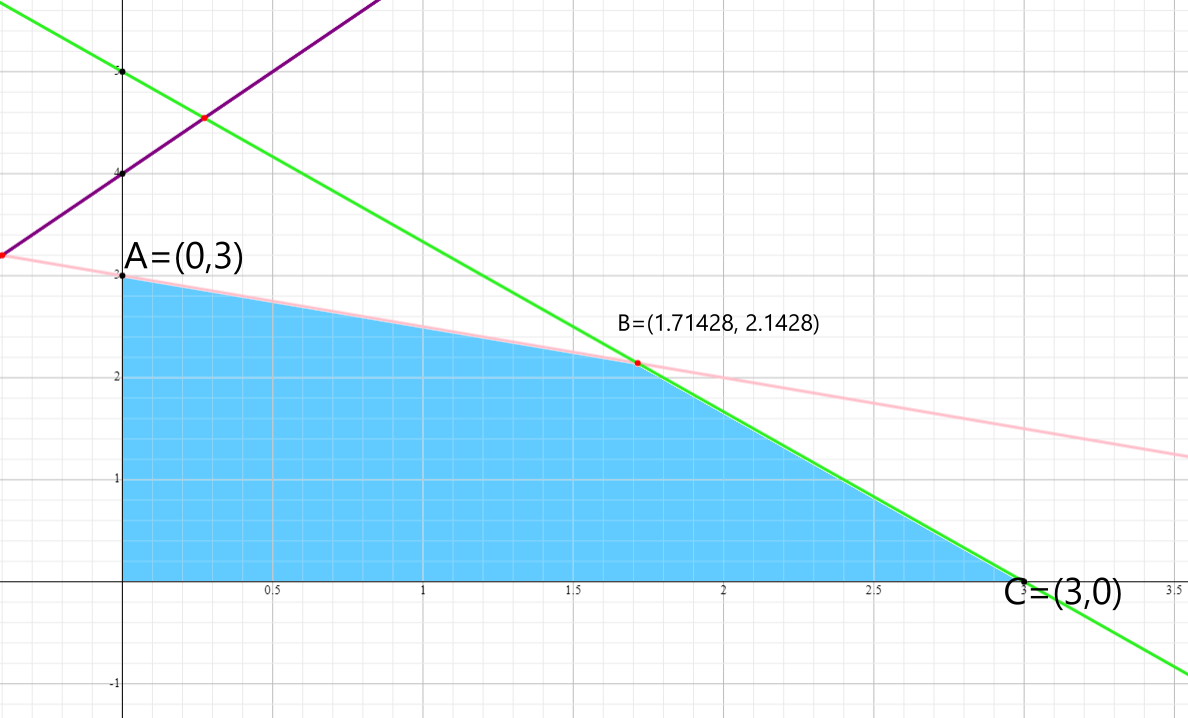
\includegraphics[scale=0.2]{Ejercicios/graficas/Ejercicio2_1.png}
    
    \item Por el método simplex\\
    \begin{tabular}{|l|l|l|l|l|l|l|l|}
\hline
Tabla 1 &   &     & 5                          & 4   & 0   & 0   & 0   \\ \hline
Base    & z & x_0 & x_1                        & x_2 & x_3 & x_4 & x_5 \\ \hline
x_3     & 0 & 6   & 1                          & 2   & 1   & 0   & 0   \\ \hline
x_4     & 0 & 4   & -2                         & 1   & 0   & 1   & 0   \\ \hline
x_5     & 0 & 15  & 5                          & 3   & 0   & 0   & 1   \\ \hline
Z       & 1 & 0   & \cellcolor[HTML]{FE0000}-5 & -4  & 0   & 0   & 0   \\ \hline
\end{tabular}
\Rightarrow
\begin{tabular}{|l|l|l|l|l|l|l|l|}
\hline
Tabla 2 &   &     & 5   & 4                           & 0   & 0   & 0    \\ \hline
Base    & Z & x_0 & x_1 & x_2                         & x_3 & x_4 & x_5  \\ \hline
x_3     & 0 & 3   & 0   & \cellcolor[HTML]{FE0000}1.4 & 1   & 0   & -0.2 \\ \hline
x_4     & 0 & 10  & 0   & 2.2                         & 0   & 1   & 0.4  \\ \hline
x_1     & 5 & 3   & 1   & 0.6                         & 0   & 0   & 0.2  \\ \hline
Z       & 1 & 15  & 0   & -1                          & 0   & 0   & 1    \\ \hline
\end{tabular}
\Rightarrow

\begin{tabular}{|l|l|l|l|l|l|l|l|}
\hline
Tabla 3 &   &                                     & 5   & 4   & 0            & 0   & 0            \\ \hline
Base    & z & x_0                                 & x_1 & x_2 & x_3          & x_4 & x_5          \\ \hline
x_2     & 4 & \cellcolor[HTML]{00D2CB}2.142857143 & 0   & 1   & 0.714285714  & 0   & -0.142857143 \\ \hline
x_4     & 0 & 5.285714286                         & 0   & 0   & -1.571428571 & 1   & 0.714285714  \\ \hline
x_1     & 5 & \cellcolor[HTML]{00D2CB}1.714285714 & 1   & 0   & -0.428571429 & 0   & 0.285714286  \\ \hline
Z       &   & \cellcolor[HTML]{FE0000}17.14285714 & 0   & 0   & 0.714285714  & 0   & 0.857142857  \\ \hline
\end{tabular}

la solución es
$$(1.7142857142857, 2.1428571428571)$$

    \item Representa en la gráfica los movimientos de cada una de las iteraciones simplex
    
    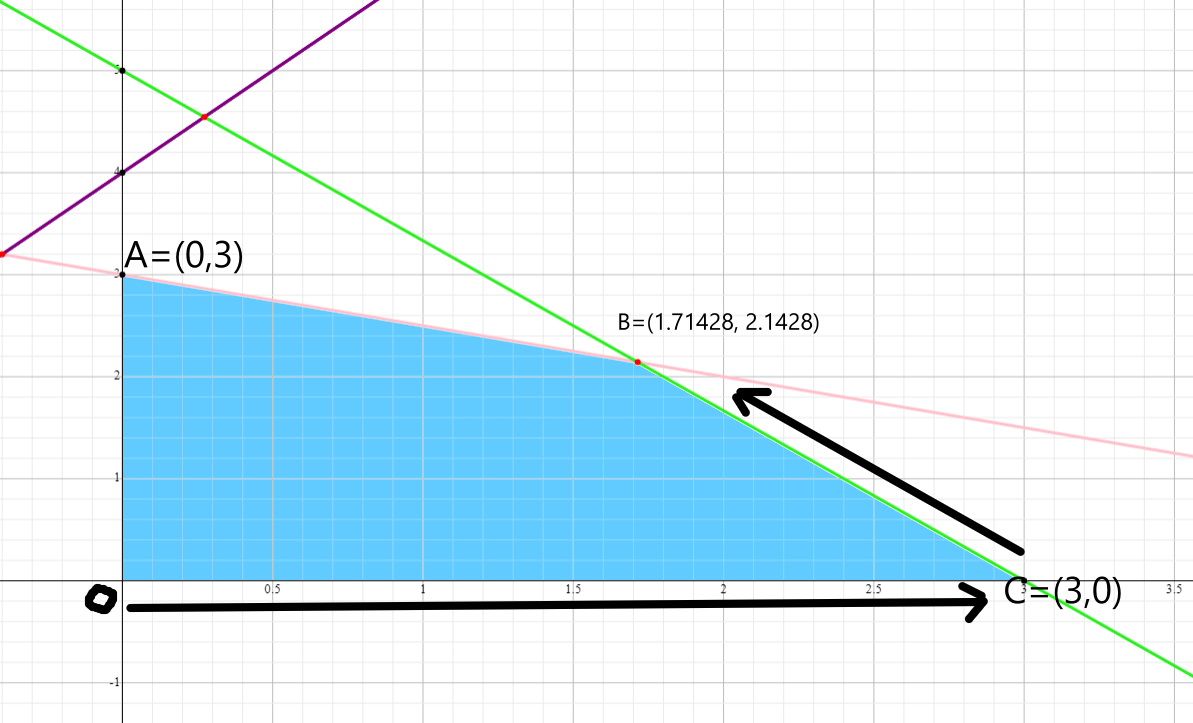
\includegraphics[scale=0.2]{Ejercicios/graficas/Ejercicio2_2.png}
    
\end{itemize}